% Do not change document class, margins, fonts, etc.
\documentclass[a4paper,oneside,bibliography=totoc]{scrbook}

% some useful packages (add more as needed)
\usepackage{scrhack}
\usepackage[utf8]{inputenc}
\usepackage{graphicx}
\usepackage{latexsym}
\usepackage{amsmath}
\usepackage{amssymb}
\usepackage{tabularx}
\usepackage{csquotes}
\usepackage{booktabs}
\usepackage{listings}
\usepackage{algorithm}
\counterwithin{algorithm}{chapter}
\usepackage{algorithmic}
\usepackage{csquotes}
\renewcommand{\algorithmiccomment}[1]{\hfill\textit{// #1}}
\usepackage[usenames,dvipsnames]{xcolor}
\usepackage[colorlinks,citecolor=Green]{hyperref}
\usepackage{lipsum}
\usepackage[printonlyused]{acronym}

% chicago citation style
\usepackage{natbib}
\bibliographystyle{chicagoa}
\setcitestyle{authoryear,round,semicolon,aysep={},yysep={,}} \let\cite\citep

% example enviroments (add more as needed)
\newtheorem{definition}{Definition} \newtheorem{proposition}{Proposition}

% Definition einer Turtle‑Sprache
\lstdefinelanguage{Turtle}{
  morekeywords={@prefix,@base,a},
  morekeywords=[2]{ex,exp,rdfs},
  morestring=[b]",
  morestring=[b]',
  sensitive=true,
  basicstyle=\small\ttfamily,
  keywordstyle=\color{blue},
  keywordstyle=[2]\color{magenta},
  commentstyle=\color{gray}\itshape,
  stringstyle=\color{OliveGreen},
  columns=fullflexible,
  breaklines=true,
  breakatwhitespace=false,
  literate={:}{{{\color{orange}:}}}1,
}

% Definition einer SPARQL‑Sprache
\lstdefinelanguage{SPARQL}{
  morekeywords={@prefix,@base,a,SELECT,WHERE},
  morekeywords=[2]{ex,exp,rdfs},
  morestring=[b]",
  morestring=[b]',
  sensitive=true,
  basicstyle=\small\ttfamily,
  keywordstyle=\color{blue},
  keywordstyle=[2]\color{magenta},
  commentstyle=\color{gray}\itshape,
  stringstyle=\color{OliveGreen},
  columns=fullflexible,
  breaklines=true,
  breakatwhitespace=false,
  literate={:}{{{\color{orange}:}}}1,
}

% Globales Styling für alle Listings
\lstset{
  language=Turtle,
  frame=single,
  numbers=left,
  numberstyle=\tiny\color{gray},
  numbersep=5pt,
  tabsize=2,
  captionpos=b,
  basicstyle=\small\ttfamily,
}

\begin{document}

\frontmatter
\subject{Master Thesis}
\title{Title of Your Master Thesis}
\author{Max Lautenbach\\
  (matriculation number XXXXXXXX)}
\date{\today}
\publishers{{\small Submitted to}\\
  Data and Web Science Group\\
  Dr.\ Sven Hertling\\
  University of Mannheim\\}
\maketitle

\chapter{Abstract}

% Your abstract goes here

\begingroup%
\hypersetup{hidelinks}%
\tableofcontents%
\endgroup

\chapter{List of Abbreviations}
\begin{acronym}
  \acro{AI}{Artificial Intelligence}
  \acro{CRM}{Customer Relationship Management}
  \acro{LLM}{Large Language Model}
  \acro{MAS}{Multi-Agent System}
  \acro{ML}{Machine Learning}
  \acro{OWL}{Web Ontology Language}
  \acro{RAG}{Retrieval Augmented Generation}
  \acro{RDF}{Resource Description Framework}
  \acro{RDFS}{Resource Description Framework Schema}
  \acro{SPARQL}{SPARQL Protocol and RDF Query Language}
  \acro{URI}{Uniform Resource Identifier}
  \acro{VDBMS}{Vector Database Management System}
  \acro{DBMS}{Database Management System}
  \acro{GPT}{Generative Pre-trained Transformer}
  \acro{LLaMA}{Large Language Model Meta AI}
  \acro{LM}{Language Model}
\end{acronym}

\mainmatter

\chapter{Introduction}
\label{ch:intro}

% Your introduction goes here

\chapter{Background}
\label{ch:related_work}
In the following chapter, the necessary theoretical background to understand core concepts of this approach will be described. Therefore, the chapter will start with an explanation of knowledge graphs (section \ref{sec:knowledge_graphs}). Building on that foundation, a section on closed information extraction (section \ref{sec:closed_information_extraction}), which is the problem that is approached in this work, will follow. Afterwards the theoretical background on the multi-agent-system approach will be defined starting with the core language and embedding models alognside with the retrieval augmented generation use case (section \ref{sec:language_models}, \ref{sec:sentence_embeddings} and \ref{sec:retrieval_augmented_generation}) over to defining what \ac{AI} agents and multi-agent-systems are (section \ref{sec:ai_agents} and \ref{sec:multi_agent_systems}), leading to a section on agent design best practises (section \ref{sec:agent_design}).
\section{Knowledge Graphs}
\label{sec:knowledge_graphs}
Knowledge graphs are a concept to store knowledge in a way that the semantic in the knowledge is machine-retrievable \cite{GomezPerez2017}. In order to accomplish this goal, knowledge graphs are directed graphs, whereas the nodes define real world entities and the edges define the relationsship between the entities \cite{Paulheim2016}. To define the domain and give a knowledge graph a set of rules, the types of entities and relations are predefined in what is called an ontology \cite{GomezPerez2017,Paulheim2016}. Following those definition, the ecosystem of knowledge graphs is build from three building blocks: knowledge graph construction, knowledge graph storage, knowledge graph consumption \cite{GomezPerez2017}.

Starting from the construction, knowledge graphs are represented in \ac{RDF}, which is the standard to represent knowledge graphs. \ac{RDF} is build of triples, whereas each triple could be seen as description of a relation by the three parts \textit{Start Node, Edge and Target Node}. All parts of the triple are either a resource identifier, a blank node or a literal. In the case of this work, the used resource identifier is a \ac{URI} like for example \textit{\url{http://example.org/entity/Angela_Merkel}}, that is why all chapters the term \ac{URI} will used consisent instead of change to more general or more specific identifiers. Exception to the general denotation by \acp{URI} are blank nodes and literals. Blank nodes is a concept where a resource could not be specified. This could be the case, if the relation that is described by the triple includes concepts like \textit{someone} or \textit{something}. Literals are simple values, like integers or strings \cite{VillazonTerrazas2017}.

The relation described by the triples can also be seen as a simple english sentence consisting of subject matching the start node, predicate matching the edge and object matching the target node. For each of those there are common rules, when defining the knowledge graph. Subjects can be either an \ac{URI} or a blank node. Predicates, which are called properties from now on as predicates are named properties throughout in knowledge graphs, can only be \acp{URI}. An Object can be an \ac{URI}, a blank node or a literal. Inheriting this concept the \ac{RDF} contains multiple syntactical representations of knowledge graphs, one of which Turtle is \cite{VillazonTerrazas2017}.

Turtle is build up of simple triple statements consisting of subject, property and object, where each part is separated by either a space, tabluation or whitespace. Each statement in turtle is terminated like a normal sentence using a dot. A \ac{URI} must be enclosed in angle brackets, whereas blank nodes can be represented with an underscore follow with a colon and an arbitrary name for the blank node instead of a \ac{URI} and Literals are enclosed in quote, where turtle interpreter either define the datatype of the value themselves or the datatype can be defined by the user. In the follow example, it can be seen how four sentences can be defined within the turtle format \cite{Tomaszuk2020}.


\begin{lstlisting}[language=Turtle, caption=Example of a Knowledge Graph in Turtle Format, label=lst:turtle_example, escapechar=@]
@\textcolor{gray}{\# Angela Merkel is member of the CDU.}@
<http://example.org/entity/Angela_Merkel> <http://example.org/property/member_of> <http://example.org/entity/CDU>.

@\textcolor{gray}{\# Angela Merkel is written "Angela Merkel".}@
<http://example.org/entity/Angela_Merkel> <http://www.w3.org/2000/01/rdf-schema#label> "Angela Merkel".

@\textcolor{gray}{\# Angela Merkel is greeted by someone.}@
<http://example.org/entity/Angela_Merkel> <http://example.org/property/greeted_by> _:b1.

@\textcolor{gray}{\# This someone works for Friedrich Merz.}@
_:b1 <http://example.org/property/works_for> <http://example.org/entity/Friedrich_Merz>.
\end{lstlisting}

In order to simplify the turtle statements, prefixes can be defined. Those prefixes corralate to a namespace, which is a path in the \ac{URI} which multiple resource are stored under. A prefix is defined using \textit{@prefix}, the name of the prefix followed by a colon (i.e. \textit{ex:}) and the namespace itself. In the shown example using prefixes could simplify the turtle statements to the following \cite{Tomaszuk2020}:

\begin{lstlisting}[language=Turtle, caption=Example of a Knowledge Graph in Turtle Format, label=lst:turtle_example]
@prefix ex: <http://example.org/entity/>
@prefix exp: <http://example.org/property/>
@prefix rdfs: <http://www.w3.org/2000/01/rdf-schema#>

ex:Angela_Merkel exp:member_of ex:CDU.
ex:Angela_Merkel rdfs:label "Angela Merkel".
ex:Angela_Merkel exp:greeted_by _:b1.
_:b1 exp:works_for ex:Friedrich_Merz.
\end{lstlisting}

Besides defining the entities and their relationship, turtle is also used to implement ontologies. In general ontologies can be defined using \ac{RDFS} or \ac{OWL}, which itself is an extension to \ac{RDFS}. The idea behind \ac{RDFS} is to provide a standardised way to define classes and properties for a knowledge graph. In addition, \ac{RDFS} can make the semantic of a knowledge graph more extensive by providing restrictions or indents on a class. One apparent restrictions is the domains and ranges attached on properties. Domains and ranges are type restrictions on the subject (domain) and object (range) of a triple. When there is a property like \textit{exp:member\_of} is defined, the ontology can hold the domain \textit{ex:human} and the range \textit{ex:organisation}, which means the every subject \textit{S} that is member of an object \textit{O} must be of type \textit{ex:human}, whereas the object must be of type \textit{ex:organisation}. As \ac{RDFS} is limited in experessive power, \ac{OWL} was developed as extension providing ideas like symmetric properties like \textit{exp:married\_to}, which when A is married to B, we can imply that B is married to A. \ac{OWL} also provides an extensive set of possible restrictions, which opens the opportunity to design complex restrictions on either classes or properties \cite{VillazonTerrazas2017}.

Following up to the building block of knowledge graph construction, it is necessary to introduce triple stores as the building block of knowledge graph storage. Triple stores are build to save and retrieve identities form a triplex collection, which means that triple stores are connection construction and retrieval. The triplex collection has to comply with the \ac{RDF} standard \cite{Rusher2003}. One triple store implementation is Apache Jena. Jena provides a whole triple store stack, allowing to manipulate and retrieve an \ac{RDF} graph via API or direct I/O modules in Java. In addition, Jena supports all mentioned standard like \ac{RDF}, \ac{RDFS} and \ac{OWL} \cite{Carroll2004}. To support the de-facto standard knowledge graph query language \ac{SPARQL} \cite{VillazonTerrazas2017}, the Apache Jena Toolset implements Jena Fuseki which is working as a \ac{SPARQL} server \cite{Chokshi2022}.

The idea of \ac{SPARQL} is to retrieve data from a \ac{RDF} knowledge graph, but also to manipulate data in it. The language is following the standards of turtle, when it comes to query construction. Three most essential query types are select, ask and insert queries. Select queries are able to retrieve content from the graph. Ask queries are simplified select queries, that can just acknowledge on an existance of the requested query. Insert queries are ones to manipulate the data in the graph \cite{VillazonTerrazas2017}.

In general a \ac{SPARQL} query begins with the query type followed with the \textit{WHERE} keyword and the query definition. In the case of select queries, the query type keyword is followed by variables, which are defined be a leading question mark followed by the variable name (i.e. \textit{?organisation}). As \ac{SPARQL} follows the turtle language also prefixes can be defined. In addition \ac{SPARQL} queries can take filtering and query options like limits or offsets \cite{VillazonTerrazas2017}. To show an example, if you want to search the organisations Angela Merkel is member of, a \ac{SPARQL} query could look like this:

\begin{lstlisting}[language=SPARQL, caption=Example of a SPARQL Query, label=lst:turtle_example]
  @prefix ex: <http://example.org/entity/>
  @prefix exp: <http://example.org/property/>
  
  SELECT ?organisation WHERE {
    ex:Angela_Merkel exp:member_of ?organisation
  }
  \end{lstlisting}

As all building blocks of a knowledge graphs are declared, the goal is now to introduce one use case of knowledge graphs to show the capabilities but also challenges in leveraging knowledge graphs in real world use cases. A project named HAVAS 18 aimed to monitor start-up activities, tech trends and tech talents leveraging knowledge graphs. This comes by leveraging existing relationships between the mentioned entities on social networks. This could reveal relevant relations and create a better understanding how start-ups, tech trends and tech talents arise and evolve. As social networks can already provide structured relationship data, the data basis of the knowledge graph can be extracted \cite{Monti2017}. On the other side \citet{Monti2017} states, that the main challenges of this project were entity resolution and disambiguation as well as the processing of unstructured data. This already shows up challenges, that this work tries to solve.

In addition to such specific use cases, there are approaches, which try to represent the largest online encyclopoedia Wikipedia into a knowledge graph. Two present approaches are Wikidata and DBpedia. The goal of Wikidata was to establish a knowledge management for factual information in Wikipedia. Leveraging knowledge graph technology the idea was to eliminate redundancies and create multi-language support. Therefore, Wikidata is also a community-based project, where the community can make changes in the graph. In addition, Wikidata is nowadays the factual information knowledge store integrated into Wikipedia \cite{Vrandecic2014}. In addition, DBpedia is another knowledge graph employed to provide data for semantic web applications. Other than in Wikidata, DBpedia use extraction frameworks leveraging syntactical structured constructs from MediaWiki to convert Wikipedia dumps to \ac{RDF}.

As a conclusion, knowledge graphs can provide semantically rich data, by leveraging the graph data structure together with standardised frameworks and languages build around the knowledge graph concept. In addition, knowledge graphs are publically available in immense size and are open to use. Nevertheless, when developing use cases utilising knowledge graphs, the challenges could come down to process unstructured data and detect ambiguated entities.

\section{Closed Information Extraction}
\label{sec:closed_information_extraction}
Closed information extraction is the problem area of extracting triples out of an unstructured text, whereas each part of triple must match the underlying knowledge graph \cite{Josifoski2021}. This means that the extracted entities and properties have to match the exact string, that can be mapped into the knowledge graph. This differs from open information extraction, as there the textual information gets convert in free-form triples \cite{Etzioni2008}.
Another concept in the area of information extraction is relation extraction, which is focussed on identifying the relation between entities, which also includes detecting entities \cite{Zhao2024}. Relation extraction differs from open relation extraction, as the type and structure of relations are already defined \cite{Kamp2023}. All problems are sub-problems of the field of information extraction, which is defined as the general process to extract entities and relations out of a text \cite{Etzioni2008}.

As especially relation extraction and closed information extraction share many similarities, the challenges and solutions are also similar. The first challenge is about to identify and extract entities out of a text. From there on, entities can be already linked to a knowledge graph in the case of closed information extraction. In this case entity extraction necessarily means also entity disambiguation, as there might be entities using the same name in the knowledge graph. Using the identified entities, relations must be detected between them and those relations have to be classified. Afterwards a mapping of those relations into the knowledge graph must be done when processing a closed information extraction task \cite{Josifoski2021,Zhao2024}.

To process those tasks, there are two approaches: A pipeline or a joint-approach. The pipeline approaches work through those tasks step-by-step. In some cases the exact steps are variied as tasks can be splited up or joined. In joint approaches all steps happen at the same time but implicitly. This is an approach to reduce error propagation throughout the single steps in the pipelines by combining them, in order to optimised methods towards the overall target of producing correct triples \cite{Zhao2024,Josifoski2021}.

Whereas the ideas of all subproblems of information extraction remains the same, \citet{Josifoski2021} states, that especially open information extraction techniques are not applicable to closed information extraction. This is grounded in the complexity of closed information extraction, being constraint to a knowledge base. Therefore, closed information extraction requires structured output that is ready to be mapped onto entities and properties in a knowledge graph \cite{Josifoski2021}.

Overall closed information extraction is a very restricted subclass of information extraction where the additional challenge of mapping entities and properties to a knowledge base is added to the remaining challenges. Those challenges are covering entity extraction, disambiguation and linking together with the actual relation extraction and linking. Each of this steps can produce errors, which is why either pipeline approaches are used, where each step is tried to be as error-resistant as possible or joint approaches are used, which can be optimised towards the overall goal.

\section{Language Models}
\label{sec:language_models}
A \ac{LM} is a \ac{ML} model, that at its core is able to predict the probabilities of how a text is going to be completed based on the previous text\cite{Radford2019}. Since the original publication by \citet{Vaswani2023} most present \acp{LM} are build out of two components, the tokenizer and the transformel model. The tokenizer transforms parts of a text into a integers. Therefore, the integers are like a index in a vocabulary mapping a character sequence to an integer \cite{Sennrich2016}. In present models like the GPT-models the existing tokenizer is a byte-pair encoding \cite{Radford2019}. This byte-pair encoding works by intialising a vocabulary using single characters. Afterwards frequent character sequences will be merged iteratively, create new tokens. This will be done until a defined maximum number of tokens in the vocabulary is reached \cite{Sennrich2016}. With that explained, a \ac{LM} can be mathematically formulated as a conditional probability $P$ of the token $t_i$ under the condition of all previous tokens:
\begin{equation}
  P(t_i|t_1,...,t_{i-1}).
\end{equation}

The core part of a \ac{LM} is the transformer. Transformers itself are \ac{ML} models that concept of Multi-Head-Attention Layers and Feed-Fordward Layers. Attention is a concept to encode previously tokens ($t_1,...,t_{i-1}$) and their relation to the current token $t_i$ into the encoded representation of the current token. The implementation of this concepts requires an learned embedidng of all tokens and three learnable weight matrices. An embedding is in this case a trained mathematical representation of a token. The weight matrices split up in one weight matrix $W^Q$ for the current token and two weight matrices $W^K, W^V$ for the previous tokens \cite{Vaswani2023}. The idea behind this concept is, that those weight matrices are able to detect relations like adjectives and therefore influence the encoding of a token \cite{Sanderson2024}. For instance, when the text \enquote{... the former german chancelor Angela Merkel ...} is processed by the attention layer, the attention mechanism could encode \enquote{former german} into the token of \enquote{chancelor}. It has to be mentioned, that this is an example and the exact behavior of the attention layer could differ \cite{Sanderson2024}.

Following this idea, \citet{Vaswani2023} proposed the concept of multi-head attention to learn multiple weight matrices and run the matrix multiplication done by the attention mechanism multiple times in parallel. Afterwards the result of all attention heads are concatenated and projected using the Softmax function \cite{Vaswani2023}. Therefore, multi-head attention could also be able to identify various kinds of relationships inside a sentence \cite{Sanderson2024}. In addition to multi-head attention, a position encoding is inserted into the embeddings of the tokens \cite{Vaswani2023}. In addition, each output of the attention respective the feed forward layer gets added to the initial input to this layer and afterwards get normalized. The Transformer is completed by a linear layer mapping the vector representation back on the vocabulary and a softmax layer to get a probability distribution across the vocabulary \cite{Vaswani2023}. Figure \ref{fig:transformer} shows the overall composition of transformers with the encoder component on the left and the decoder component on the right. As following explanations focusses on the already explained components the masked-multi-head-attention and encoder-decoder split will not be covered.

\begin{figure}[h]
  \centering
  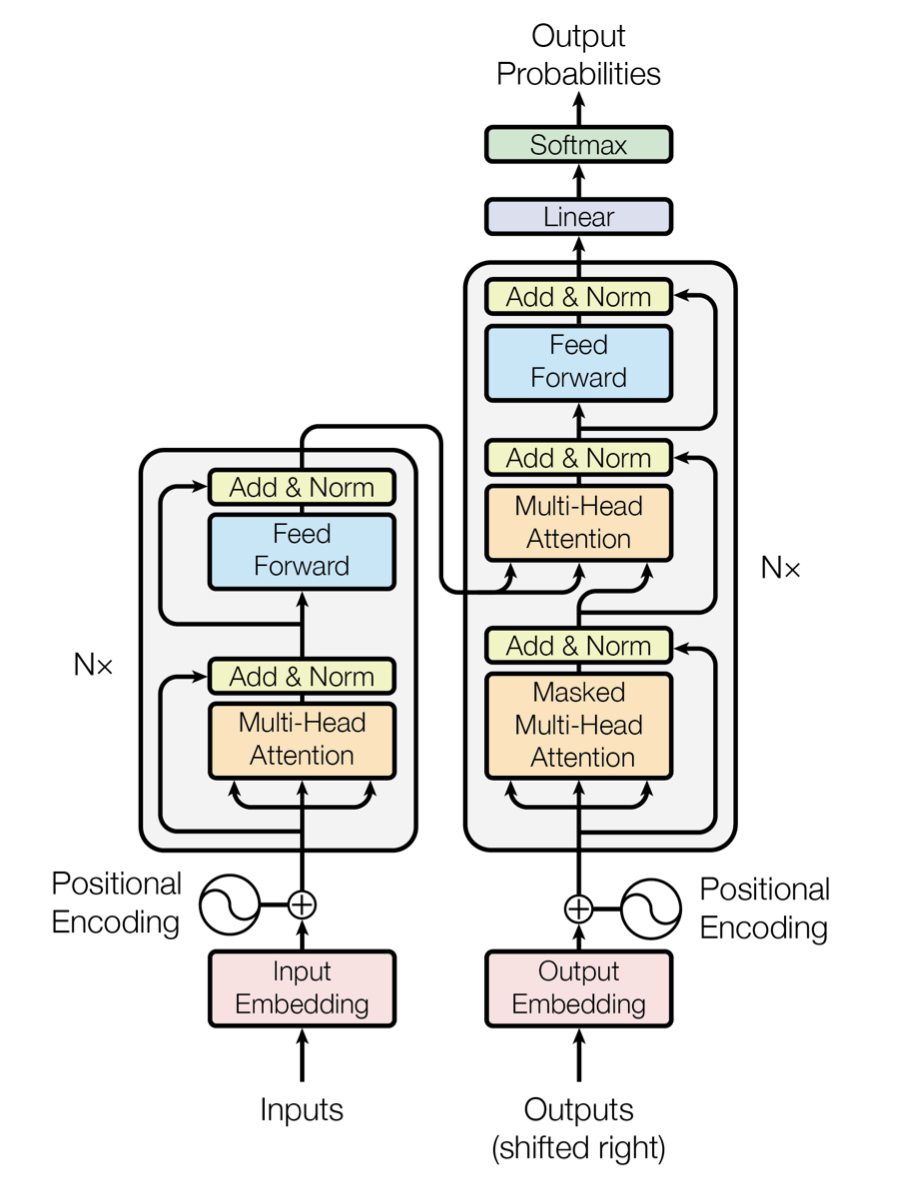
\includegraphics[width=0.5\textwidth]{figures/Transformer.png}
  \caption{Architecture of a Transformer model. \cite{Vaswani2023}}
  \label{fig:transformer}
\end{figure}

As already stated, a softmax function is used to get a probability distribution across all possible output tokens. Normally the sampling process of the next token is used to be a random process, where each tokens has the assigned weight from the softmax function. In order to increase or decrease randomness, a temperature parameter $T$ is introduced in the softmax function \cite{Peeperkorn2024}. For each output $z_i$ on token $t_i$ for a sequence with length $n$ the softmax function $softmax(\mathbf{z})_i$ with the temperature $T$ will be calculated as \cite{Peeperkorn2024}:

\begin{equation}
  softmax(\mathbf{z})_i = \frac{exp(\frac{z_i}{T})}{\sum^n_j exp(\frac{z_j}{T})}~~~where~\mathbf{z} \in \mathbb{R}^n.
\end{equation}

Increasing the temperature $T>1$ would lower high probabilities and increase low probabilities and therefore make the output more novel in theory. A temperatur $T<1$ would amplify high probabilities and make the text generation more predictable. Using a temperature $T=0$ change the generation to greedy sampling, as then only the token with the highest probability is used \cite{Peeperkorn2024}.

Todays top-tier like OpenAIs \ac{GPT} models or Metas \ac{LLaMA} models \acp{LM} do make use of the decoder part of the transformer \cite{Radford2018,Grattafiori2024}. Models especially with large amount of parameters are typically referred to as \acp{LLM}. Those decoder-only models do only have the target to make predictions for the token $t_i$. Those models use unsupervised pre-training, by using a text-corpora and maximizing the probabilities of each subsequent token in this corpora to be predicted. In former models like the original GPT version, after pre-training a task-specific supervised fine-tuning was necessary to get usable results \cite{Radford2018}.

The recent history of \acp{LM} showed, that increasing the corpora size on the pre-training and the parameters number enables the models to be able to process tasks from various domains without further fine-tuning \cite{Radford2018,Radford2019,Brown2020}. With the GPT-3 publication, \citet{Brown2020} showed that their model can leverage in-context learning to increase their performance on specific tasks. Therefore, in the input of the model, what is also called the prompt, examples will be added. For instance, when the \ac{LM} should process translation tasks, it get's in it's prompt examples like \textit{house $\rightarrow$ Haus} or \textit{light bulb $\rightarrow$ Glühbirne}. Including multiple examples is called few-shot prompting, while including one example is called one-shot-prompting and including no example is called zero-shot prompting.

This technique has shown great success especially when using larger models, as they were able to process in-context information more efficient. But also the zero-shot experiments showed superior performance to SOTA models in various tasks, showing the general capabilities of recent \acp{LM} \cite{Brown2020}. To enable this performance, \citet{Brown2020} used the Common Crawl corpora, filtered it and added also other smaller, but high quality corpora to their pre-training dataset. Therefore, the \ac{GPT}-3 pre-training dataset had access on over 500 billion tokens \cite{Brown2020}.

As the Common Crawl corpora follows the idea of providing a copy of the entire internet \cite{CCF2025} and other used corpora also provide prose text combined with the overall training goal of \acp{LM} leads to a superior performance in text generation but not in instruction following \cite{Ouyang2022}. In addition, \citet{Ouyang2022} states the real-world usage of \acp{LM} differ from the given corpora, as most users use instructions. Therefore, \ac{GPT}-3 was finetuned towards two datasets. One dataset uses human-given answers to prompts to fine-tune the model. In addition, human-labeled comparisons between answers of different \ac{GPT}-3 models are used to train a reward models, that is applied using reinforcement learning on the model. At the end of the experiements, the resulting InstructGPT model reached superior performance on human evaluated benchmarks based on the output on held-out prompts from customers. Even the smallest instruction tuned model with 1.3 billion parameters outperformed \ac{GPT}-3 with 175 billion parameters in this evaluation \cite{Ouyang2022}.

In order to choose ideal model for use-cases, on option could be to use benchmarks like MMLU-Pro \cite{Wang2024} or the human-evaluated Chatbot Arena \cite{Chiang2024}. The MMLU-Pro benchmark is testing for multi-task language understanding with the goal to test the various capabilities of LLMs. Therefore, the MMLU-Pro keeps tasks from maths, physics, law, engineering and various other topics \cite{Wang2024}. The Chatbot Arena\footnote{The Chatbot Arena can be accessed under \url{https://lmarena.ai}} is a live benchmark working with human preferences. Therefore, the use gets two answers from two distinct models to the user prompt. Then the human chooses which \ac{LM} performed better. Based on this feedback a win rate and a score can be calculated \cite{Chiang2024}.

In conclusion, \acp{LM} are \ac{ML} models consisting out of multiple multi-head attention and feed-forward network layers with the goal to predict the probability of a following token based on all previous tokens. Therefore, those models are designed as with a large amount of parameters and additional use pre-training based on large size corpora to achieve outperforming results. In the end, those models can be benchmarked using MMLU-Pro or the Chatbot Arena to test various capabilities of them.

\section{Sentence Embeddings}
\label{sec:sentence_embeddings}

Sentence embeddings in general have the idea to represent a text in a vector \cite{Singhal2001}. Building those vectors, the semantic of the sentence can be encoded in those embeddings, so that a meaningful similarity between the vectors can be calculated \cite{Reimers2019}. Typically this similarity is the cosine of the angle between two vectors, which is named cosine similarity. The property of the cosine function then allows, that the cosine between two vectors is 1.0 when they are total identical and 0.0 if not \cite{Singhal2001}. Such models are critical to enable large-scale semantic similarity comparisons which are useful for various use cases, like retrieving knowledge similar to a user query \cite{Reimers2019,Gao2024}.

One recent model is M3-Embedding, which is trained to support semantic retrieval functions that rely on similarity functions. The overall idea of M3-Embedding is to support multiple languages, multiple retrieval functionalities and multiple input granularities. To achieve this goal M3-Embedding leverage the encoder architecture of transformers like stated in section \ref{sec:language_models} \cite{Chen2024}.

Training-wise, \citet{Chen2024} follows the pre-training approach, while fine-tuning later on high-quality data. The pre-training was done on unlabeled corpora utilising semantic structures like title-body or title-abstract. To support multi-linugua a translation dataset was leveraged. Then labeled corpora in different languages and synthesised corpora consisting of questions generated by \ac{GPT}-3.5 based on multilingual paragraphs were used to fine-tune the embeddings. Overall the M3-Embedding model was trained to detect if a queries matches a text passage from its semantics or not \cite{Chen2024}.

Overall sentence embeddings can be used to map sentence into the vector space, while also encoding semantic into this space. Leveraging vector algebra like the cosine similarity, semantic similarity between two sentence embeddings can be calculate. To achieve SOTA performance embeddings like M3-Embedding make use of the transformer architecture combined with extensive training sets and the pre-training technique.

\section{Retrieval Augmented Generation}
\label{sec:retrieval_augmented_generation}

As \acp{LM} are trained on large-size snapshots of corpora, they are by default not able to retrieve out-of-scope knowledge from the internal representation. Therefore, \ac{RAG} emerged as a solution to incorporate knowledge from external data sources into the \ac{LM} at runtime. \ac{RAG} in it's simplest form is build out of indexing, retrieval and generation. In the indexing step, the plain text, also called document, will be mapped into the vector space utilising embedding models like the previously named M3-Embeddings \cite{Gao2024}. This embeddings are stored for later retreive in a database that can handle vectors and vector algebra efficient \cite{Gao2024,Pan2024}.

The steps of retrieval and generation are done at runtime, whereas the indexing can run independend. The retrieval steps utilises again the embedding model to map the user query into the vector space. As shown in section \ref{sec:sentence_embeddings}, models like M3-Embeddings are trained on to calculate the similarity between documents and user queries. This enables the retrieval step to run a similarity search on the \ac{VDBMS} and retrieve the most relevant documents based on the user query. After the retrieval those documents can be composed into a prompt template, where additionaly to the user prompt, a system prompt can be defined. Then this prompt is send to the \ac{LM} with the goal to produce a external knowledge aware answer \cite{Gao2024}.

Besides the already explained embeddings the \ac{RAG} depends on a \ac{VDBMS}. Those databases consist like normal \ac{DBMS} out of a query processor and a storage manager. The query processor is optimising the query and processes especially the similarity searches. One example of \ac{VDBMS} is Qdrant. Qdrant uses filtering and vector set size depended execution paths. If a vector set, named collection in Qdrant, keeps many vectors, a brute-force search would be to extensive. Therefore, Qdrant would use pre-filtering mechanism that limit the search results and computations that have to be done. The storage manager manages the physical access and storage of the data \cite{Pan2024}.

As already stated Qdrant is an example for a \ac{VDBMS}. It uses the concept of collection, where vectors are stored that should be retrieved together, for instance to cluster vectors that all belong to one project. Additionally to the vectors, payloads can be used to store metadata alongside with the vectors. Qdrant offers a python client and a Langchain integration, which is useful to be leveraged in vector store projects \cite{Qdrant2025}. Langchain itself is a framework to develop application with \acp{LM} \cite{LangChain2025d}. Through its query optimisations, Qdrant is able to handle large-scale datasets efficient \cite{Qdrant2025,Pan2024}.

\ac{RAG} is one solution to integrate external knowledge bases, that can be updated efficient, into \acp{LM}. Therefore, \ac{RAG} makes use of the ability of embeddings to encode semantic similarity that can be retrieved using cosine similarity. In order to make use of \ac{RAG} the external knowledge bases have to be indexed using embeddings. To support \ac{RAG}, \ac{VDBMS} are utilised for an efficient indexing and retrieval process.

\section{AI Agents}
\label{sec:ai_agents}

\ac{AI} agents are a more narrow concept of a normal agent. \citet{Dorri2018} defines an agent as \enquote{(a)n entity which is placed in an environment and senses different parameters that are used to make a decision based on the goal of the entity. The entity performs the necessary action on the environment based on this decision.} \cite[S. 28574]{Dorri2018} The entity in this case is defined as the type of the agent. The enviroment is the place of the agent, which is defined by the accessibility and quality of data, predictability of outcomes, the dynamic of enviroment changes and continuity of the state. Parameters can be defined as the data that the agent gets and the action is the set of actions that the agent can take \cite{Dorri2018}.

Agents do have a decision engine. \ac{AI} agents typically narrow this decision engine nowadays down to \acp{LLM} \cite{Sapkota2025,Park2023}. Furthermore \ac{AI} agents are defined by having a high degree of idependence, while being task-specific and react and adapt to the current state \cite{Sapkota2025,OpenAI2025}. The high degree of independence differs to workflows, were the path how to achieve a goal is well-defined \cite{Anthropic2024}. The idea behind \acp{LLM} that power agents is to generate human-like behavior, as \acp{LLM} have internal representation of human behavior via the training data \cite{Park2023}.

To achieve this goal the agent architecture cosists of agent orchestration, a \ac{LLM} model used for decision making and reasoning and tools \cite{Wiesinger2025,OpenAI2025}. All components are executed by an agent runtime. The orchestration layer is the layer that defines which information an agent gets. This consists of managing memory, providing the prompt templates to the agent and define a message flow, so how the actions that the agent takes are executed \cite{Wiesinger2025}.

According to \citet{OpenAI2025} tools can be defined in three types: Data, Action, Orchestration. Data tools are concentrated on retrieving information from external systems. Therefore, data tools can query databases or search the web. Action tools enable the agent to take actions in external systems. This means, the agent could update or create record in systems like a \ac{CRM}. Orchestration agents, agents that serve themselve as tools. This concept is referred to as \ac{MAS} an will be explained in detail in section \ref{sec:multi_agent_systems}. In general, tools are an enabler to AI agent to directly interact with external systems. This interaction allows \ac{AI} agents to act highly idenpendent.

A single \ac{AI} agent is targeted to process a single well defined tasks together with defined tools. Within this task it stays indepent, but a single \ac{AI} agent is not offering a high degree of flexibility, when not using other agents as tools \cite{Sapkota2025}. In this use case \citet{Anthropic2024} proposes that \ac{AI} agents are able to understand complex inputs, can make use of tools in reliable manner and recover from errors. In addition, \ac{AI} agents can engage in reasoning and planning over given tasks \cite{Anthropic2024}.

The ability to reason is especially used in the ReAct agent framework proposed by \citet{Yao2023}. The idea behind the ReAct frame is the synergy between reasoning on perceptions and taking action from there on, as this is a typical learning behavior of humans. In the proposed idea, the \ac{LLM} is mocking this human behavior by being told to reason and act \cite{Yao2023}.

In general the ReAct framework prompts an \ac{LLM} to reason about a task using a defined state. The resulting thought will be written in the state, alongside with all following thought. Besides giving a thought, the \ac{LLM} is prompted to take an action which could either be running a tool, running itself again or ending the process. This action leads to a result which is called observation. After each thought in the state, an action and the following observation is stored. Together this build up a history, that the \ac{LLM} could leverage to memorise it's own thoughts and actions \cite{Yao2023}.

To implement \ac{AI} agents \citet{Anthropic2024} proposes to take a framework like LangGraph. LangGraph is an open-source frame to build agent with the whole agent ecosystem. Therefore, tools, memory and the state can be define either using LangGraph in python or JavaScript. LangGraph offers a high extensibility, to define the agent as individual as needed \cite{LangChain2025}. Alltogether LangGraph is integrated with the LangChain package \cite{LangChain2025a}.

Single agents bring challenges along. First of all there are limitations brought by the \ac{LLM}, which is about missing the understanding for causal relationships. This arises out of the goal to generate text instead of detection causal relationships. In addition, as \acp{LLM} are prompt sensitive, the overall outcome is prompt sensitve \cite{Sapkota2025}. Furthermore, \citet{Sapkota2025} states, that \ac{AI} agents have limited long-horizon planning and missing recovery mechanism leading them to get stuck in a loop.

Overall \ac{AI} agents are defined by a model taking independent actions. Therefore, an agent must be orchestrated and has access to various tools. The ReAct framework can implement the ideas and capabilities of \ac{AI} agents so that the \acp{LLM} behave human-like and therefore achieve good results.

\section{Multi-Agent-Systems}
\label{sec:multi_agent_systems}

As stated in the previous section agents are often limited to a single task, being unflexible to solve other tasks. A solution to this limitation can be found in \ac{MAS}. The idea behind them is to produce a cost efficient, flexible and reliable solution, by using multiple agents instead of one. Therefore, the complex task can be splitted into multile simple task. The theory is that the simpler task lead to lower cost solutions amortising the overhead produced to manage the \ac{MAS} \cite{Dorri2018}.

So to make a general \ac{MAS} work, agents are defined for various simpler task. In addition, multiple agents could be defined for the same task. Then the routing within the \ac{MAS} must be defined. This means, that there is either a static or dynamic topology of agent and the communication routes between them. In this topology there coould a leader agent, that defines the actions that have to be taken by other agents and they communicate solely to the leader. The second option is a leaderless \ac{MAS}, where each agent decide on its on which agent is to call next \cite{Dorri2018}.

Especially leaderless \ac{MAS} bring a high degree of flexibility with them. From this, a high complexity arises in coordinating the agents towards one shared goal, organising the agents to communicate to each other and allocating a task to the correct agent with the correct inputs. Additionally, as multiple agents conduct to one goal, fault propagation and fault detection is getting more complex \cite{Dorri2018}.

All mentioned points can also be mapped and extended when focussing on \ac{LLM} based \ac{MAS}. In general, due to the capabilities of \acp{LLM}, single \ac{AI} agents are already able to take care of complex tasks. But the only way to keep with more complex task is to increase instruction size and the number of tools, which could lead the \ac{AI} agents into failing or looping like already outlined in section \ref{sec:ai_agents} \cite{OpenAI2025}. Therefore, the goal decomposition into various specialised \ac{AI} agents remains also a key enable to solve more complex tasks \cite{Sapkota2025}.

In the case of \ac{LLM}-based \ac{MAS}, each agent is in general required the same building blocks like mentioned in section \ref{sec:ai_agents}. This concept is adapted to \ac{MAS} by extending the state to a shared state \cite{Sapkota2025}. In addition, each agent in a \ac{MAS} needs to have an handoff. This handoff is defined by the agent itself and decides the further flow within agent system. Especially in LangGraph the handoff specifies the destination of the handoff, so the next tool or agent, and the payload, meaning the update of the state or inputs to the next agent or tool. Therefore, the orchestration layer of the \ac{LLM}-based \ac{MAS} gets more complex, what could be handled by frameworks like LangGraph \cite{LangChain2025b}.

The agentic architecture patterns of a \ac{LLM}-based \ac{MAS} follows the classic \ac{MAS} patterns. The leader-follow pattern is defined as supervisor pattern by \citet{LangChain2025b}, alongside with the hierarchical pattern. The supervisor pattern therefore, has on supervisor agents, that manages the communication to other expert agents, which themselve can only communicate with the supervisor agent. In the hierarchical pattern, those expert agent can itself be supervisors to other expert agents \cite{LangChain2025b}.

\ac{LLM}-based \ac{MAS} can also be used with decentralised leaderless architecture \cite{OpenAI2025,LangChain2025b}. This concept is extended by \citet{LangChain2025b} to network and custom patterns. The network pattern allows each agent to decide to which agent in the network it should handoff its request. In this pattern each agent controls the flow within the \ac{MAS} \cite{LangChain2025b,OpenAI2025}. The custom pattern could not be perfectly adapted to either leader-follow nor leaderless patterns. In the custom pattern a user can also define workflows for specific agents or let some agents not communicate with specified other agents \cite{LangChain2025b}. The big benefit besides the theoretical more accurate performance of \ac{LLM}-based \ac{MAS}, is the high modularity that is being enabled. In addition, through packages like LangGraph, the communication flow between the agents can be precisely defined alongside with the agents specialisation \cite{LangChain2025b}.

Nevertheless, \ac{LLM}-based \ac{MAS} amplifies and adds challenges that were already apparent with \ac{AI} agents. At first within \ac{LLM}-based \ac{MAS} the lack of causal understanding gets amplified, as agents have to run multiple times. Each \ac{AI} agent brings already uncertainty with them, especially being prompt sensitive and are vulnerable to infinite loops. Using multiple \ac{AI} agents, leads to even more uncertainty and robustness \cite{Sapkota2025}. In addition, the communication and coordination of \ac{LLM}-based \ac{MAS} reveals further bottlenecks. This is amplified by the fact, that \acp{LLM} have limited context length model-wise and infrastructure-wise \cite{Kwon2023}. This adds complexity in managing shared context and aligning on one goal \cite{Sapkota2025,Han2025}. As \acp{LLM} can produce unpredicted behavior, \ac{LLM}-based \ac{MAS} is non-composable. This means, that adding another \ac{AI} agent to a \ac{LLM}-based \ac{MAS} could lead to more complexity in the prompts, but it does not necessarily mean, that this new agent is used. Therefore, new agents could decrease the overall performance of the \ac{MAS}. In addtion, with further scaling and the prompt senstivity of \acp{LLM} it remains complex to detect the root causes of issues in the \ac{MAS}. An evolving challenge is the immature foundations and the reletavely new reasearch field aroun \acp{LLM} in general, but especially in \ac{AI} agents and \ac{LLM}-based \ac{MAS} \cite{Sapkota2025}.

As this research subject is rapidly evolving, also solutions are already found towards several problems. For instance to support \acp{LLM} in better reasoning, one way is to include external knowledge bases using \ac{RAG}. In addition, as a \ac{LLM}-based \ac{MAS} also use \ac{AI} agents, those agent can also access tools, which are deterministic and deliver reliable results. The root cause tracing issue can be solved by using monitoring and auditing tools. In order to give \acp{LLM} a way to sense causality by using complex simulation-tools. The communication bottlenecks can also be solved using different memory architectures \cite{Sapkota2025}.

Overall \ac{LLM}-based \ac{MAS} are one solution to solve complex problems efficient and accurate. Therefore, multiple \ac{AI} agents, that solve one piece of the overall problem, can communicate and take action. This could be done within a network of \ac{AI} agents, hierarchical solutions or fully custom solutions. Nevertheless, as the overhead increases and so does the \ac{LLM} calls, \ac{LLM}-based \ac{MAS} are vulnerable to challenges like uncertainty amplification or tracibility issues. As the research field is relatively new, also several solutions like tracibility tooling or uncertainty reduction by external knowledge and tool use evolved.

\section{Agent Design}
\label{sec:agent_design}
\begin{itemize}
  \item Building effective agents \cite{Anthropic2024}
  \item Prompt Engineering \cite{Schulhoff2025}
\end{itemize}

\chapter{Related Work}
\label{ch:related_work_chapter}
\begin{itemize}
  \item What Models or Work do exists in the cIE and MAS Context?
  \item What Dataset do exist in the cIE Context? How are they compared? How are they extracted?
  \item GenIE \cite{Josifoski2021}
  \item synthIE (Model and Dataset) \cite{Josifoski2023}
  \item REBEL (Model and Dataset) \cite{HuguetCabot2021}
  \item DISCIE \cite{Moeller2024}
  \item AgentRE \cite{Shi2024}
\end{itemize}

% Your literature review goes here

\chapter{Approach}
\label{ch:approach}
\section{Agent Architectures}
\label{sec:agent_architectures}
\subsection{Baseline}
\label{subsec:baseline}
\subsection{Supervisor}
\label{subsec:supervisor}
\subsection{ReAct}
\label{subsec:react}
\subsection{Network}
\label{subsec:network}

\section{Agent Tools}
\label{sec:agent_tools}
\subsection{URI Search}
\label{subsec:uri_search}
\subsection{Network Traversal}
\label{subsec:network_traversal}
\subsection{Message Deletion}
\label{subsec:message_deletion}
\subsection{Semantic Validation}
\label{subsec:semantic_validation}
\subsection{Turtle to Label}
\label{subsec:turtle_to_label}
\section{Evaluation Setup}
\label{sec:evaluation_setup}
\subsection{Dataset}
\label{sec:dataset}
\begin{itemize}
  \item synthIE
\end{itemize}
\subsection{Wikidata}
\label{sec:wikidata}
\begin{itemize}
  \item How does Wikidata looks like?
\end{itemize}
\begin{itemize}
  \item Langgraph
  \item 2 Datasplits on synthIE Text (Train Val, Test)
  \item 2 Datasplits on synthIE Code (Train , Test) (optional)
  \item Results on 5/50 Examples
  \item Cerebras, SambaNova Cloud, vLLM on 2x A100
  \item Models: Llama 3.3 70B (Mainly), Tests with o3-mini, Llama 4 ...
\end{itemize}
% Your first main chapter goes here
\section{Language Models}
\begin{itemize}
  \item Llama 3.3 70B
  \item Gemma 3 27B
  \item Llama 4 Maverick
\end{itemize}

\chapter{Evaluation}
\label{ch:evaluation}
\section{Evaluation Metrics}
\label{sec:evaluation_metrics}
\begin{itemize}
  \item Definition Positive/Negative Triple \cite{Josifoski2021}
  \item F1-Score, Precision, Recall
  \item With Parents, With Related
\end{itemize}


\section{Evaluation Configurations}
\label{sec:evaluation_configurations}
\subsection{Initial Baseline Setup}
\label{subsec:initial_baseline_setup}
\begin{itemize}
  \item Supervisor Agent
  \item Entity Extractor
  \item Relation Extractor
  \item URI Retrieval Agent
\end{itemize}

\subsection{Modularization of Agent Tasks}
\label{subsec:modularization_agent_tasks}
\begin{itemize}
  \item Decomposition of the Supervisor Agent into:
        \begin{itemize}
          \item Planner
          \item Agent Instructor
          \item Result Checker
          \item Result Formatter
        \end{itemize}

  \item Introduction of URI-Search Filters (On Label OR Description)
\end{itemize}

\subsection{Error Message Incorporation}
\label{subsec:error_message_incorporation}
\begin{itemize}
  \item Integration of error messages
  \item Improved state monitoring and feedback
  \item Predicate Extractor in Gen1
  \item Baseline extended with URI Response Summary
\end{itemize}

\subsection{Task Simplification and State Refinement}
\label{subsec:task_simplification_state_refinement}
\begin{itemize}
  \item Simplification of agent state representations (e.g., Gen1 → Gen1v2)
\end{itemize}

\subsection{One-Agent Architecture with Tool Usage}
\label{subsec:one_agent_architecture_tool_usage}
\begin{itemize}
  \item Centralization of all tasks into a single agent
  \item Use of external tools to perform sub-tasks
\end{itemize}

\subsection{URI Retrieval Filtering}
\label{subsec:uri_retrieval_filtering}
\begin{itemize}
  \item Switch to Filtering on Entities and Properties
\end{itemize}

\subsection{Knowledge Graph Integration}
\label{subsec:knowledge_graph_integration}
\begin{itemize}
  \item Incorporation of domain-specific knowledge via:
        \begin{itemize}
          \item Network Traversal (and why deleted later)

        \end{itemize}
\end{itemize}

\subsection{Full Network Agent Architecture}
\label{subsec:full_network_agent_architecture}
\begin{itemize}
  \item Combination of insights from Baseline, Gen1, and One-Agent approaches
  \item Network-based collaboration between specialized agents
  \item Dynamic use of tools and agent interactions
  \item Few-Shot Prompting
  \item Update URI Search Modes
  \item Semantic Validation
  \item Turtle to Label conversion
\end{itemize}

\subsection{Performance Increases of Gen2 to One Agent and Baseline Architecture}
\label{subsec:performance_increases_gen2}
\begin{itemize}
  \item One Agent
  \item Baseline
\end{itemize}

\subsection{LLM Model Variation}
\label{subsec:llm_model_variation}
\begin{itemize}
  \item Various models at various stages and show results
  \item Elaborate on why to choose Llama 3.3 70B over other models
\end{itemize}

\section{Discussion}
\label{sec:discussion}


\chapter{Conclusion and Outlook}
\label{ch:conclusion_outlook}

% Your conclusions go here

\bibliography{references/references}

\appendix
\chapter{Additional Material}
\label{ch:additional_material}

% Your additional material goes here

\backmatter
\chapter{Ehrenwörtliche Erklärung}
\label{ch:declaration}

Ich versichere, dass ich die beiliegende Bachelor-, Master-, Seminar-, oder
Projektarbeit ohne Hilfe Dritter und ohne Benutzung anderer als der angegebenen
Quellen und in der untenstehenden Tabelle angegebenen Hilfsmittel angefertigt
und die den benutzten Quellen wörtlich oder inhaltlich entnommenen Stellen als
solche kenntlich gemacht habe. Diese Arbeit hat in gleicher oder ähnlicher Form
noch keiner Prüfungsbehörde vorgelegen. Ich bin mir bewusst, dass eine falsche
Erklärung rechtliche Folgen haben wird.

\begin{center}
  \textbf{Declaration of Used AI Tools} \\[.3em]
  \begin{tabularx}{\textwidth}{lXlc}
    \toprule
    Tool & Purpose & Where? & Useful? \\
    \midrule
    % Add your AI tools here
    \bottomrule
  \end{tabularx}
\end{center}

\vspace{2cm}
\noindent Unterschrift\\
\noindent Mannheim, den XX.~XXXX 2024 \hfill

\end{document}
